\documentclass[11pt]{article}

\usepackage[margin=1in]{geometry}
\usepackage{amsfonts, amsmath, amssymb}
\usepackage[none]{hyphenat}
\usepackage{fancyhdr}
\usepackage{graphicx}
\usepackage{float}
\usepackage[nottoc, notlot, notlof]{tocbibind}
\usepackage{hyperref} %for clickable links

\pagestyle{fancy}
\fancyhead{}
\fancyfoot{}
\fancyhead[L]{\slshape \MakeUppercase{Radio}}
\fancyhead[R]{\slshape Modeling}
\fancyfoot[C]{\thepage}
%\renewcommand{\headrulewidth}{0pt} %to remove the horizontal line in header
\renewcommand{\footrulewidth}{0pt} %to remove the horizontal line in footer

\parindent 0ex %removes paragraph indentation
%\setlength{\parindent}{4em} %change the width of the indent
%\setlength{\parskip}{1em} %change the amount of spacing between paragraphs
\renewcommand{\baselinestretch}{1.5} %affects line spacing of paragraphs 

\begin{document}

\begin{titlepage}
\begin{center}
\vspace*{1cm}
\Large{\textbf{Software Modeling}}\\
\Large{\textbf{Modeling and Implementation Phase}}
\vfill
\line(1,0){400}\\[1mm]
\huge{\textbf{“Radio Simulator”}}\\[3mm]
\Large{\textbf{- Models -}}\\[1mm]
\line(1,0){400}\\
\vfill
By ESSAFSYFY Abdelkrim and MELUZOLA KIMFUTA Gingu\\
Academic year 2019-2020
%Candidate \#\\

\end{center}
\end{titlepage}

\tableofcontents
\thispagestyle{empty} %removes header and footer from table of contents
\clearpage %table of content on its own page
\setcounter{page}{1} %1st page is after table of contents

Note that both models are in an "alpha" version, which means that they are subject to change in the future (implementation phase).

\section{Configurator}
\vspace{20px}
\begin{center}
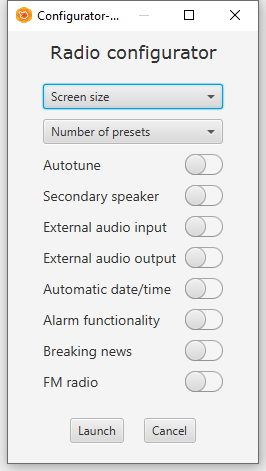
\includegraphics[width=5cm]{../Screenshots/configurator-v3.png}\\
\end{center}
Before launching the radio itself, we must choose what functionalities are available and what are not. In order to do that, the first window we encounter when launching the simulation is the radio configurator.\\
The configurator allows the selection and variation of the radio type:
\begin{itemize}
\item Screen size selection (small, medium or large) which changes the amount of data displayed
\item Number of presets available (ranging from 3 to 10)
\item Enable or disable optional features from the secondary dashboard (see Use case diagram in diagrams report)
\end{itemize}


\section{Radio}
As mentioned above, the configurator allows for three types of displays: large, medium and small. The only difference is the amount of information displayed in the radio screen. In order to reduce the amount of figures, we assume that every functionality has been chosen in the configurator.
\subsection{Large screen size}
\vspace{10px}
\begin{center}
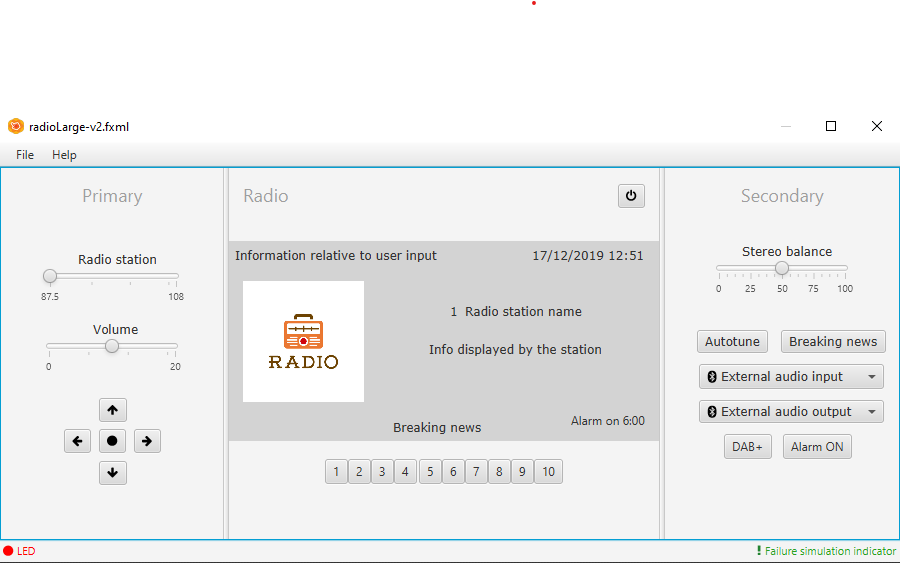
\includegraphics[width=15cm]{../Screenshots/radioLarge-v4.png}\\
\end{center}
When choosing all the available functionalities and a large screen, we are met with the window above.\\
Going from top left to bottom right, we will discuss the different window elements throughout the report:
\begin{itemize}
\item Menu: File: contains multiple options such as:
\begin{itemize}
\item Failure simulation: allows to test and observe the radio's behavior following different types of malfunctions.
\item Back to configurator: allows to go back to the configurator in order to use a different type of radio without having to close the window and restart the simulation.
\item Breaking news: simulate a breaking news broadcast from the currently selected station
\end{itemize}
\item Menu: Help: contains information about the radio, simplified user manual and miscellaneous informations.
\item Primary: the primary functionalities the radio has, they come in every radio regardless of its screen size; radio station selection slider, volume slider and navigation controls. The latter has many uses. Please refer to the use cases' description in the diagrams report for detailed description. We will briefly enumerate these uses:
\begin{enumerate}
\item Choose what information is displayed in the monitor: the user uses the four arrows to navigate the screen, the selected text is highlighted. It is possible to hide or show the information using the center button.
\item Change the date and time
\item Set the alarm time
\end{enumerate}
\item The 10 preset buttons are displayed in the center of the window despite being part of the primary dashboard, this is simply a design choice.
\item Power button: allows to turn the radio on of off, the LED indicator bellow changes accordingly.
\end{itemize}

\subsection{Medium screen size}
\vspace{10px}
\begin{center}
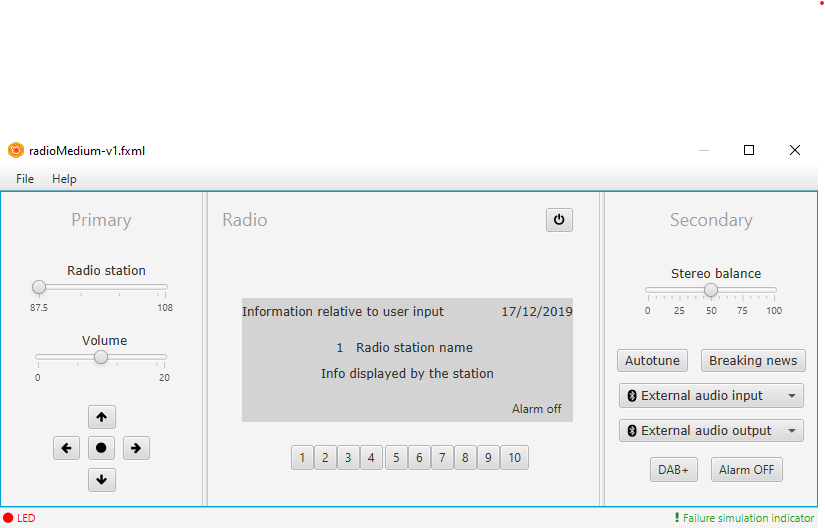
\includegraphics[width=15cm]{../Screenshots/radioMedium-v2.png}\\
\end{center}
When choosing a medium screen size, we can no longer see the radio station's image and breaking news. In this case the user can only hide/display the initially available information (they can not show the radio's image since it does not exist due to the limited screen size). Moving on to the screen display:
\begin{itemize}
\item Top left: the relative information to the user's input. For example: if the user changes the volume, the radio displays the information here.
\item Top right: the current date and time
\item Center: the radio station's number and name followed, underneath it, by its informations.
\item Center left: the radio station's image (logo, ad, ...)
\item Bottom center: breaking news, which are only displayed when receiving the information from the radio channel.
\item Bottom left: alarm status (on/off) and the time it is set to.
\end{itemize}

\subsection{Small screen size}
\vspace{10px}
\begin{center}
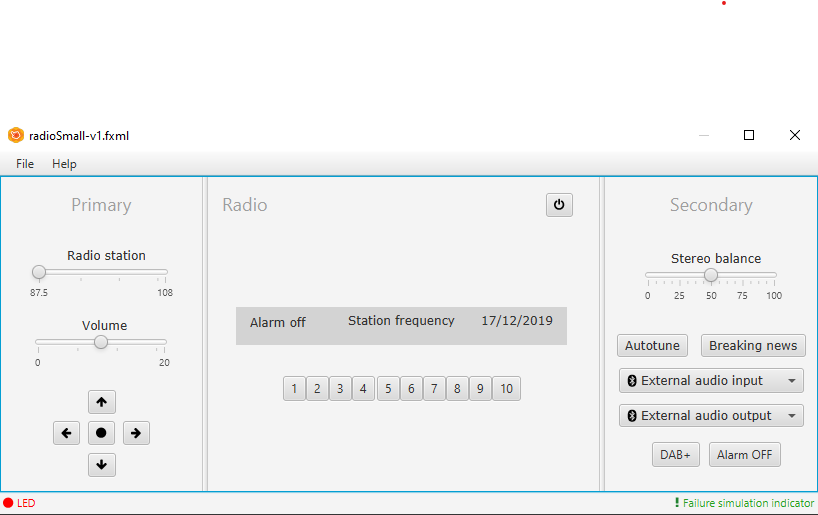
\includegraphics[width=15cm]{../Screenshots/radioSmall-v2.png}\\
\end{center}
When choosing a small screen size, the only available information in the screen is the radio station's name and the date and time.\\ The secondary dashboard contains the optional features chosen in the configurator:
\begin{itemize}
\item Stereo balance: allows the user to balance the audio between left and right speaker
\item Autotune and breaking news
\item External audio input: allows the user to plug in an external audio input allowing the radio to receive sound from an external device. There are three choices (USB, audio jack and bluetooth)
\item External audio output: allows the user to plug in an external audio output allowing the radio to redirect the sound to external speakers. There are two choices. (audio jack and bluetooth)
\item DAB+: allows to switch from DAB+ to FM standard and vice versa.
\item Alarm ON/OFF: activate or deactivate the alarm.
\item Failure simulation indicator: displays the state of the radio following a simulated malfunction.
\end{itemize}


\end{document}